\section[Tema]{Tema}
Il diabete si configura come uno dei disturbi di natura cronica più ampiamente diffusi all'interno del panorama sanitario degli Stati Uniti, coinvolgendo annualmente un considerevole numero di cittadini americani e gravando pesantemente sull'economia nazionale. 
Tale condizione costituisce una patologia di natura cronica, la cui gravità risiede nella perdita da parte degli individui della capacità di gestire efficacemente i livelli di glucosio presenti nel circolo ematico, con il risultato di una possibile riduzione della qualità della vita e dell'aspettativa di vita.
In seguito al processo di digestione, durante il quale vari alimenti vengono trasformati in zuccheri, questi ultimi trovano via libera nel flusso sanguigno, innescando una risposta del pancreas che conduce alla liberazione dell'insulina.
Quest'ultima svolge un ruolo cruciale nell'agevolare l'utilizzo degli zuccheri da parte delle cellule dell'organismo per soddisfare il fabbisogno energetico. 
La sintomatologia del diabete si caratterizza, in genere, per l'inadeguata produzione d'insulina da parte dell'organismo o per una scarsa capacità di utilizzare l'insulina prodotta in maniera efficiente.

Le complicazioni, quali le affezioni cardiache, la compromissione della vista, l'amputazione degli arti inferiori e i disturbi renali, sono strettamente correlate ai livelli cronici eccessivi di zucchero presenti nel circolo sanguigno dei soggetti affetti da diabete.
Tali complicanze impongono un peso aggiuntivo sulla vita quotidiana di coloro che convivono con questa patologia, riducendo la qualità della vita e limitando l'aspettativa di vita. 
Nonostante la mancanza di una cura definitiva, esistono diverse strategie di gestione che consentono di mitigare gli effetti nocivi di questa patologia in un numero considerevole di pazienti.
La perdita di peso, un regime alimentare sano, l'attività fisica regolare e l'impiego di trattamenti medici mirati rappresentano alcune delle misure di prevenzione e gestione efficaci per contrastare il diabete.
La diagnosi precoce gioca un ruolo chiave in questo contesto, permettendo l'adozione tempestiva di modifiche nello stile di vita e l'avvio di trattamenti più efficaci, circostanza che rende i modelli predittivi del rischio di diabete strumenti di fondamentale importanza per gli operatori del settore sanitario pubblico.

È imprescindibile cogliere l'ampiezza di questo problema.
Secondo quanto riferito dai \textit{Centers for Disease Control and Prevention} (CDC), nel 2018 ben 34,2 milioni di cittadini americani erano affetti da diabete, mentre 88 milioni presentavano una condizione di prediabete.
Questi numeri sottolineano la vastità del problema e la sua diffusione su scala nazionale.
Inoltre, il CDC stima che uno su cinque soggetti affetti da diabete e circa otti su dieci individui con prediabete ignorino il proprio stato di rischio.
La mancanza di consapevolezza riguardo al rischio di sviluppare il diabete rappresenta una sfida significativa per la prevenzione e la gestione di questa patologia.
È pertanto necessario intensificare gli sforzi di informazione e sensibilizzazione per promuovere la consapevolezza sulla prevenzione del diabete.

Pur esistendo varie forme di diabete, il diabete di tipo II rappresenta la variante più comune e la sua incidenza varia in relazione a fattori quali età, istruzione, reddito, posizione geografica, razza e altri elementi determinanti dell'aspetto salutistico.
Il fatto che il diabete abbia una diffusione differenziata in base a questi fattori mette in evidenza la complessità e la diversità del problema.
In particolare, i dati evidenziano che le comunità con un basso reddito e un livello di istruzione più limitato tendono a sperimentare una maggiore prevalenza del diabete.
In questo contesto, emerge la necessità di affrontare il diabete da una prospettiva di giustizia sociale, garantendo l'accesso alle risorse e alle informazioni necessarie a tutte le fasce della popolazione.

Non va trascurato il fatto che il peso di questa patologia si riversa preponderantemente sui soggetti con un basso livello di sviluppo socioeconomico.
Il diabete impone altresì un gravoso onere economico, con costi diagnostici associati al diabete stimati a circa 327 miliardi di dollari e costi totali, che comprendono il diabete non diagnosticato e il prediabete, che si attestano intorno ai 400 miliardi di dollari annui \cite{diabetesEconomics}.
Questi costi rappresentano una considerevole spesa per il sistema sanitario e l'economia nazionale, sottolineando ulteriormente l'importanza di investire nella prevenzione, nella diagnosi precoce e nella gestione efficace del diabete.
Gli sforzi per ridurre il costo sociale ed economico del diabete devono essere basati su strategie di prevenzione e sul miglioramento dell'accesso a cure efficaci, allo scopo di ridurre il numero di casi di diabete e migliorare la gestione delle condizioni esistenti.

\section[Dataset]{Dataset}
Il \textit{Behavioral Risk Factor Surveillance System} (SSFR) è un sondaggio telefonico correlato alla salute raccolto annualmente dai \textit{Centers for Disease Control and Prevention}.
Ogni anno, il sondaggio raccoglie le risposte di oltre 400.000 cittadini americani su comportamenti a rischio per la salute, condizioni croniche di salute e l'utilizzo di servizi preventivi.
Questa iniziativa è stata avviata ininterrottamente dal 1984.
Per questo progetto, è stato utilizzato un file CSV del set di dati disponibile su Kaggle relativo all'anno 2015 \cite{dataset}. \\
Questo set di dati contiene le risposte di 441.455 individui e comprende 330 caratteristiche.
Queste caratteristiche sono rappresentate sia da domande direttamente rivolte ai partecipanti, sia da variabili calcolate sulla base delle risposte individuali dei partecipanti.

Il dataset utilizzato per lo studio in questo software è "\textit{diabetes-binary-5050split-health-indicators-BRFSS2015.csv}", un insieme di dati pulito composto da 70.692 risposte a un sondaggio condotto dal CDC nell'anno 2015, noto come \textit{BRFSS2015}. \\
Il dataset presenta una distribuzione equa del 50-50 tra i partecipanti senza diabete e coloro con prediabete o diabete.
La variabile target "\textit{Diabetes-binary}" ha 2 classi: 0 indica l'assenza di diabete, mentre 1 indica la presenza di prediabete o diabete.

Questo dataset è bilanciato e comprende 21 variabili:

\begin{longtable}{lp{2cm}p{8cm}}
  \toprule
  \textbf{Nome Variabile} & \textbf{Valori} & \textbf{Descrizione} \\
  \midrule
  \endfirsthead
  \multicolumn{3}{l}{{Continua dalla pagina precedente}} \\
  \toprule
  \textbf{Nome Variabile} & \textbf{Valori} & \textbf{Descrizione} \\
  \midrule
  \endhead
  \bottomrule
  \multicolumn{3}{r}{{Continua nella pagina successiva}} \\
  \endfoot
  \bottomrule
  \caption{Descrizione delle variabili nel dataset.}
  \endlastfoot
  HighBP & 0, 1 & Presenza di alta pressione \\
  HighChol & 0, 1 & Presenza di colesterolo alto \\
  CholCheck & 0, 1 & Controllo del colesterolo negli ultimi 5 anni \\
  BMI & & Indice di Massa Corporea \\
  Smoker & 0, 1 & Fumatore (almeno 100 sigarette nella vita) \\
  Stroke & 0, 1 & Presenza di ictus \\
  HeartDiseaseorAttack & 0, 1 & Presenza di malattia coronarica o infarto miocardico \\
  PhysActivity & 0, 1 & Pratica di attività fisica negli ultimi 30 giorni \\
  Fruits & 0, 1 & Consumo quotidiano di frutta \\
  Veggies & 0, 1 & Consumo quotidiano di verdure \\
  HvyAlcoholConsump & 0, 1 & Consumo pesante di alcol \\
  AnyHealthcare & 0, 1 & Presenza di copertura sanitaria \\
  NoDocbcCost & 0, 1 & Impedimento a vedere un medico per motivi economici \\
  GenHlth & 1-5 & Valutazione generale della salute (scala da 1 a 5) \\
  MentHlth & 1-30 & Giorni di cattiva salute mentale (scala da 1 a 30) \\
  PhysHlth & 1-30 & Giorni di malattia fisica o lesioni negli ultimi 30 giorni (scala da 1 a 30) \\
  DiffWalk & 0, 1 & Difficoltà seria a camminare o salire le scale \\
  Sex & 0, 1 & Genere (0 = Femminile, 1 = Maschile) \\
  Age & 1-13 & Categoria di età \\
  Education & 1-6 & Livello di istruzione \\
  Income & 1-8 & Reddito \\
\end{longtable}

\subsection[Algortimi]{Algortimi ML utilizzati}

Nel contesto di questa ricerca, ci siamo dedicati all'analisi delle complesse dinamiche dei dati attraverso l'impiego di avanzati algoritmi di classificazione.

\begin{itemize}
  \item \textbf{Gradient Boosting Classifier}, abbreviato come GBTClassifier, è un potente algoritmo di apprendimento automatico che appartiene alla categoria degli algoritmi di boosting.
  L'obiettivo principale di GBTClassifier è costruire un modello predittivo attraverso l'aggregazione sequenziale di modelli più deboli, generalmente alberi decisionali, ciascuno dei quali corregge gli errori del modello precedente.
  GBTClassifier migliora progressivamente la sua capacità predittiva, concentrandosi sugli errori residui del modello precedente, e integrando queste correzioni per ottenere un modello complessivamente più robusto e preciso.
  Questo processo iterativo di addestramento rende GBTClassifier particolarmente adatto per gestire dati complessi e non lineari, fornendo risultati di elevata accuratezza nelle attività di classificazione.
  La sua flessibilità e capacità di adattamento lo rendono uno strumento efficace in una varietà di contesti applicativi, dall'analisi finanziaria alla classificazione di testo e altro ancora.
  \item Il \textbf{Linear Support Vector Classifier}, o LinearSVC, è un algoritmo di classificazione che fa parte della famiglia di modelli basati sulle Support Vector Machines (SVM).
  Contrariamente a SVM non lineari, LinearSVC si focalizza sulla separazione lineare dei dati, il che significa che cerca di trovare un iperpiano nel nostro spazio di feature che meglio divide le diverse classi.
  LinearSVC si distingue per la sua efficienza nel trattare grandi quantità di dati e per la sua capacità di gestire problemi di classificazione binaria e multiclasse.
  La sua natura lineare semplifica l'interpretazione del modello e può essere particolarmente efficace in situazioni in cui la relazione tra le feature e la variabile di risposta è approssimativamente lineare.
  \item Il \textbf{RandomForestClassifier} è un potente algoritmo di apprendimento automatico che appartiene alla famiglia degli algoritmi di \textit{ensemble}, più precisamente alla categoria dei \textit{random forest} (foreste casuali).
  Questo algoritmo opera creando una serie di alberi decisionali durante il processo di addestramento e quindi combinandoli per ottenere una previsione più robusta e accurata.
  La peculiarità del RandomForestClassifier risiede nel fatto che ogni albero viene costruito in modo casuale, sia nella selezione delle feature utilizzate che nel campionamento dei dati di addestramento.
  Questo aspetto di casualità contribuisce a ridurre il rischio di \textit{overfitting} (sovradattamento) e aumenta la generalizzazione del modello.
  Durante la fase di previsione, ciascun albero contribuisce con il proprio voto, e la classe più votata diventa la previsione finale del modello.
  \item Il \textbf{DecisionTreeClassifier} è un algoritmo di apprendimento automatico che appartiene alla categoria degli alberi decisionali.
  Questo tipo di modello costruisce una struttura ad albero durante il processo di addestramento, suddividendo iterativamente il set di dati in base alle feature più informative per la classificazione.
  Il funzionamento dell'algoritmo è il seguente: inizia con un nodo radice che rappresenta l'intero set di dati, quindi seleziona la feature che meglio separa le classi.
  Il set di dati viene suddiviso in base a questa feature, generando nodi figli.
  Il processo si ripete in modo ricorsivo per ciascun nodo figlio, suddividendo ulteriormente il set di dati fino a raggiungere foglie che rappresentano le classi di output.
  Il DecisionTreeClassifier è apprezzato per la sua interpretabilità e capacità di catturare relazioni complesse nei dati.
  Tuttavia, è importante gestire il rischio di overfitting, poiché l'algoritmo potrebbe adattarsi eccessivamente ai dati di addestramento, compromettendo la generalizzazione a nuovi dati.
  \item La \textbf{Logistic Regression} (Regressione Logistica) è un algoritmo di apprendimento automatico utilizzato principalmente per problemi di classificazione binaria, sebbene possa essere esteso anche a problemi multiclasse.
  Contrariamente al nome, la Logistic Regression è impiegata per problemi di classificazione anziché di regressione.
  L'algoritmo si basa su una funzione logistica (\textit{sigmoide}) che mappa la somma ponderata delle \textit{feature} di input a un valore compreso tra 0 e 1.
  Questa mappa è interpretata come la probabilità che un'istanza appartenga alla classe positiva.
  Se la probabilità supera una soglia prestabilita (generalmente 0.5), l'istanza viene classificata come positiva; altrimenti, viene classificata come negativa.
  La Regressione Logistica è apprezzata per la sua semplicità, interpretabilità e capacità di gestire problemi di classificazione lineari.
  È ampiamente utilizzata in scenari in cui è importante comprendere il contributo relativo delle diverse feature nel processo decisionale.
  Tuttavia, è essenziale notare che la Regressione Logistica assume una relazione lineare tra le feature e il logaritmo delle odds di appartenenza a una classe, il che potrebbe non essere adeguato per problemi con relazioni complesse o non lineari.
\end{itemize}

La diversità di questi algoritmi riflette la nostra volontà di adottare un approccio poliedrico per esplorare le sfumature e le relazioni nei dati nel corso del tempo.
Attraverso questa approfondita analisi, miriamo a offrire una prospettiva completa e precisa sulle dinamiche sottostanti oggetto del nostro studio.

\section[Risultati]{Risultati del caso di studio}

All'interno del nostro corpus di analisi, troviamo un elenco esaustivo degli algoritmi di classificazione che sono stati implementati attraverso i rispettivi modelli, ciascuno associato al proprio valore di accuratezza.
La struttura di questa lista segue un formato ben definito, includendo la data di costruzione del modello, l'algoritmo utilizzato, l'indicatore di accuratezza, nonché il numero di elementi presenti sia nel set di addestramento che in quello di test.

La costruzione di ciascun modello, intrapresa in date specifiche, fornisce un punto di riferimento temporale cruciale per comprendere l'evoluzione delle tecniche di classificazione nel corso del tempo.
Ogni algoritmo impiegato viene dettagliatamente registrato, accompagnato da un indicatore di accuratezza che quantifica la sua performance.
Questo indicatore offre un'istantanea chiara dell'efficacia predittiva dell'algoritmo in questione.

La ricca documentazione degli elementi presenti nei set di addestramento e di test completa questa prospettiva, consentendo un'analisi approfondita della generalizzazione del modello oltre il suo ambiente di addestramento.
Attraverso questa metodologia dettagliata, siamo in grado di esaminare con precisione come ciascun algoritmo si è comportato in diverse fasi di sviluppo del modello, valutando la sua capacità di apprendere e generalizzare le caratteristiche distintive dei dati di training per poi applicarle in modo efficace a nuovi dati di test.
  
\begin{figure}[h]
  \centering
  \definecolor{barcolor}{RGB}{0, 102, 193} 
  \definecolor{labelcolor}{RGB}{51, 51, 51}
  
  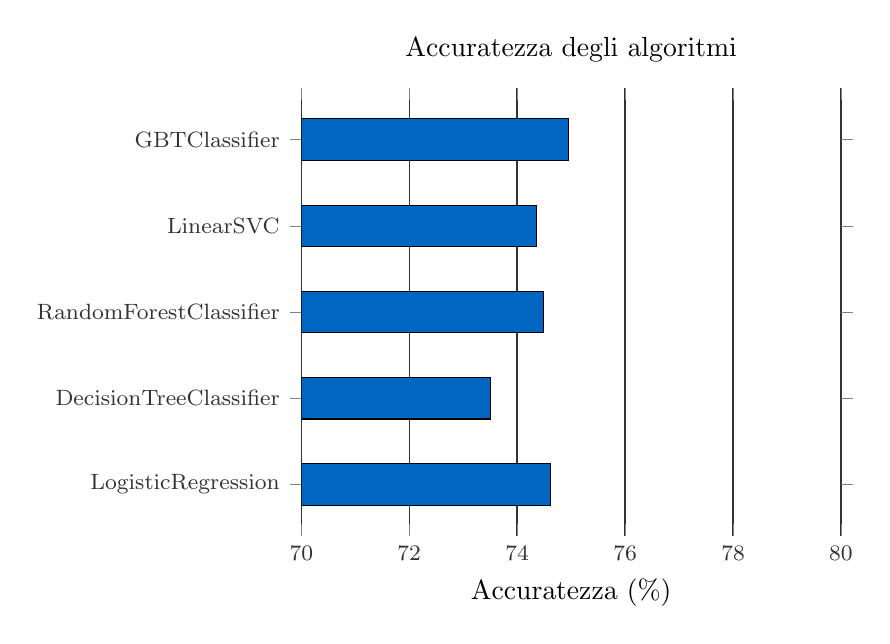
\begin{tikzpicture}
  \begin{axis}[
      title={Accuratezza degli algoritmi},
      xlabel={Accuratezza (\%)},
      symbolic y coords={LogisticRegression, DecisionTreeClassifier, RandomForestClassifier, LinearSVC, GBTClassifier},
      ytick=data,
      xbar,
      bar width=15pt,
      xmin=70, xmax=80,
      enlarge y limits=0.15, 
      legend style={at={(0.5,-0.15)}, anchor=north, legend columns=-1, draw=none}, 
      xmajorgrids=true, ymajorgrids=false,
      grid style={line width=0.5pt, color=labelcolor},
      axis line style={draw=none}, 
      tick label style={font=\footnotesize, color=labelcolor},
  ]
  
  \addplot[fill=barcolor, draw=black] coordinates {(74.61157024793389,LogisticRegression) (73.5112160566706,DecisionTreeClassifier) (74.48993949627128,RandomForestClassifier) (74.36127508854782,LinearSVC) (74.95147469582919,GBTClassifier)};
  
  \end{axis}
  \end{tikzpicture}
  \caption{Accuratezza nei dati di test per diversi algoritmi}
  \label{fig:accuratezza_algoritmi}
\end{figure}
  
  
  
  